% vim: set spell:

\chapter{Preface}

%In what follows, we give a philosophical ground for the remainder of the
%thesis. We start with imprecise notions, and arrive at precise definitions.
%Although it may seem like an imprecise ground at first, it is really a more
%honest ground than a purely ``precise'' ground. By stating the imprecise
%notions that our precise definitions build upon, we state the fundamental
%system belief which we deal within.

\section{Formal systems}

\begin{notion}

A \textbf{formal system} is a system of symbols and rules governing their
manipulation.

\end{notion}

A formal system is a purely mental construct. To be used to any effect in the
real world, a formal system must be realised by a physical system.

\begin{notion}

A \textbf{physical system} is a system of physical symbols and processes
manipulating them. 

\end{notion}

For instance, this document was typeset by a physical system. The symbols in
question are typographical symbols, and the process of typesetting is the
process of their typographic composition.

Out of considerations for the reader, the formal systems presented in this
document deal in the same typographical symbols, and govern their typographical
composition.

The reader, equipped with a writing instrument is another physical system. The
reader is welcomed to realise the formal systems in question, in attempt to
falsify the correctness of their physical realisations in this document. 

\section{Basic definitions and notation}

We begin by introducing some notation for sets, objects, and judgements,
leading to a definition of a formal system, as regarded in this document. The
matters of notation address the typesetting of this document, and bear no
logical significance otherwise.

\subsection{Sets}

\begin{definition}

A \textbf{set} is a collection of distinct elements.

\end{definition}

\begin{notation}

A typographical symbol is \textbf{distinct} from another, if the reader
can at a glance tell a difference between them.

\end{notation}

If the elements of a set can be typeset by distinct typographical symbols, the
set can be typeset elementarily by denoting the elements in a sequence. 

\begin{notation}

The elements of a set are denoted by distinct typographical symbols, which fit
inside the following box: \framebox{\vbox to 12pt {\vfil \hbox to 48pt {} \vfil
}}.

\end{notation}

\begin{notation}

A set is denoted elementarily by denoting the elements in a sequence,
left-to-right, top-to-bottom, separated by commas($,$), and enclosed in
braces($\set{}$).

\end{notation}

For instance, $\set{a,b,c}$ elementarily denotes the set containing exactly the
elements $a$, $b$, and $c$. This notational convention superimposes an order on
the elements of a set. This order bears no logical significance.

\begin{notational-corollary}

The elements of a set, when denoted elementarily in a different order, do not
denote a distinguished set.

\end{notational-corollary}

This notation is useful as it permits the reader to confirm that the elements
are distinct by considering the elements in sequence, and confirming, for each
symbol, that it does not appear more than once in the sequence. That is,
provided that the set is finite.

\begin{notion}

A set is \textbf{finite} if it can eventually be denoted elementarily.

\end{notion}

This notation does not permit to denote an infinite set, and is fairly
impractical for denoting large finite sets. To that end, the reader will be
presented with a procedure by which the elements of the set could be denoted
elementarily, had we the typographical tools and the (possibly infinite) time
to do so. The reader is then welcomed to elementarily denote the set at their
leisure. When reasoning about sets denoted by such a ``generating procedure'',
we will reason about the procedure rather than elements themselves.

\subsection{Objects}

\begin{definition}

An \textbf{alphabet} is a set.

\end{definition}

\begin{definition}

An \textbf{object} is some elements drawn from an alphabet, put in relation.

\end{definition}

\begin{notation}

An object is denoted as a typographical composition of the elements in
question, which fits within the following box:

\begin{center}
\framebox{\vbox to 48pt {\vfil \hbox to 48pt {} \vfil }}
\end{center}

\end{notation}

For instance, given the alphabet $\set{a,b,c}$, we may consider, among
others, the following objects:

\begin{center}
$abc$
\quad\quad\quad
$\begin{matrix}
  & a &   \\
a & a & a \\
  & a &
\end{matrix}$
\quad\quad\quad
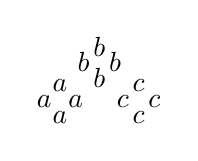
\begin{tikzpicture}
\draw (-0.5,0.0) node {$a$};
\draw (-0.7,0.2) node {$a$};
\draw (-0.3,0.2) node {$a$};
\draw (-0.5,0.4) node {$a$};
\draw (0.0,0.9) node {$b$};
\draw (0.2,0.7) node {$b$};
\draw (-0.2,0.7) node {$b$};
\draw (0.0,0.5) node {$b$};
\draw (0.5,0.0) node {$c$};
\draw (0.7,0.2) node {$c$};
\draw (0.3,0.2) node {$c$};
\draw (0.5,0.4) node {$c$};
\end{tikzpicture}

\end{center}

\begin{definition}

An object is \textbf{empty} if no symbols are drawn from the alphabet.

\end{definition}

\begin{notation}

For alphabets not containing the element $\varepsilon$, we denote the empty
object by $\varepsilon$ out of considerations for readability.

\end{notation}

\subsection{Judgements}

\begin{definition}

A \textbf{variable} is an object which is a placeholder for another object.

\end{definition}

\begin{definition}

An object is \textbf{concrete} if it is not a variable.

\end{definition}

\begin{definition}

A \textbf{judgement} is a number of concrete objects, put in relation.

\end{definition}

\begin{notation}

A judgement is a typographical combination of concrete objects, which fits
within the following box:

\begin{center}
\framebox{\vbox to 48pt {\vfil \hbox to 48pt {} \vfil }}
\end{center}

\end{notation}

Judgements come in various forms. For instance, given the objects \symb{0} and
\symb{1}, we may consider, among others, the following judgements:

\begin{table}[h!]
\centering
\begin{tabular}{|l|l|}
\hline
\textbf{Judgement} & \textbf{Reading} \\
\hline
$\symb{0}\;\text{nat}$ & \symb{0} is a natural number. \\
\hline
$\symb{1}=\symb{0}+\symb{1}$ & \symb{1} is the sum of \symb{0} and \symb{1}.\\
\hline
\end{tabular}
\end{table}

\begin{definition}

A \textbf{judgement form} is a number of objects, put in relation, some of
which may be variables.

\end{definition}

\begin{notation}

A \textbf{judgement form} is denoted as a typographical combination of the
objects in question, which fits within the following box:

\begin{center}
\framebox{\vbox to 48pt {\vfil \hbox to 48pt {} \vfil }}
\end{center}

\end{notation}

For instance, given the variables $n$, $n_1$, and $n_2$, we may consider, among
others, the following judgement forms:

\begin{table}[h!]
\centering
\begin{tabular}{|l|l|}
\hline
\textbf{Judgement form} & \textbf{Reading} \\
\hline
$n\;\text{nat}$ & $n$ is a natural number. \\
\hline
$n=n_1+n_2$ & $n$ is the sum of $n_1$ and $n_2$.\\
\hline
\end{tabular}
\end{table}

\begin{definition}

An \textbf{inference rule} is a collection of judgement forms called its
\textbf{premises} and a judgement form called its \textbf{conlusion}.

\end{definition}

\begin{notation}

An inference rule is denoted by denoting the premises in a sequence, separated
by due whitespace, over a denotation of the conclusion. The premises and
conclusion are separated by a horizontal bar.

\end{notation}

For instance, we may consider an inference rule with the single premise
$n\;\text{nat}$ and the conclusion $\symb{s}(n)\;\text{nat}$. This rule reads:
a successor of a natural number is also a natural number.

$$
\judgement[Nat-Rec]{
  n\;\text{nat}
}{
  \symb{s}(n)\;\text{nat}
}
$$

\begin{definition}

An \textbf{axiom} is an inference rule with no premises.

\end{definition}

For instance, we may consider an axiom with the conclusion
$\symb{z}\;\text{nat}$. This rules reads: zero is a natural number.

$$
\judgement[Nat-Z]{
}{
  \symb{z}\;\text{nat}
}
$$

\begin{definition}

A \textbf{judgement form} is defined by a collection of inference rules.

\end{definition}

For instance, the judgement form $n\;\text{nat}$, which reads: $n$ is a natural
number, to be defined by the rules \ruleref{Nat-Rec} and \ruleref{Nat-Z}.

\pagebreak



The procedure by which a set is elementarily denoted, is a matter of exhibiting
a procedure by which distinguished visual symbols are generated for the
elements of the set.

For instance, the natural numbers are generated from the finite alphabet
$\set{0,1,2,3,4,5,6,7,8,9}$. The first 10 symbols of $\mathbb{N}$, are just the symbols in order. The 11th symbol


\begin{definition}

A formal system $F=\chev{A,J}$ is a finite set of symbols $A$, and a finite set
of judgements $J$.

\end{definition}

% A formal system with a finite number of symbols can simulate a formal system
% with an infinite (but enumerable) number of symbols.

\begin{definition}



\end{definition}

\pagebreak

A set can be denoted elementarily, by denoting all the elements of the set, or
by exhibiting a procedure by which the elements can be denoted.


\pagebreak

% vim: set spell:

\section{Formal Systems}

\begin{notion}

A formal system, $\mathcal{F}$, is a system of symbols and rules governing
their manipulation. A symbol of $\mathcal{F}$ is distinct from all other
symbols of $\mathcal{F}$.

\end{notion}

As such, the symbols of $\mathcal{F}$ form a set:

\begin{definition}

A set is a collection of distinct elements.

\end{definition}

Formal systems are a purely mental construct. To be used to any effect in the
material world, a formal system must be realised by a physical system.

\begin{notion}

A physical system, $\mathcal{P}$, is a system of physical symbols and processes
manipulating them. A symbol of $\mathcal{P}$ is physically distinct from all
other symbols of $\mathcal{P}$.

\end{notion}

Formal systems, and so their realisations, bear little intrinsic purpose ---
symbolic manipulation is a means to an end for more purposeful beings.
Consequently, a formal system may be more, or less reasonable for a particular
purpose; a physical system may be a more, or less reasonable realisation of a
particular formal system.

The reasonability of formal systems and their realisations is a matter to be
judged by the purposeful beings themselves. This text seeks to both present the
reader with various formal systems for various purposes, and to provide
transcripts of physical systems realising them. As such, some notational
matters are in order.

\begin{notation}

The elements of a set are typographically distinct symbols.

\end{notation}

\begin{notation}

Sets are denoted in one of two ways:

\begin{enumerate}[(1)]

\item By listing the elements in sequence, separated by commas, and enclosed in
braces.  For instance $\set{\symb{a},\symb{b},\symb{c}}$ denotes the set
containing (only) the elements $\symb{a}$, $\symb{b}$, and $\symb{c}$.

\item By exhibiting a procedure by which the elements can be listed in sequence
using paper and pencil.

\end{enumerate}

\end{notation}

To each consequent symbol in the sequence, we may assign a consequent

\begin{remark}

This representation of sets superimposes an order on the elements of a set. In
particular, the order of an element of the set, is position of the element in
the sequence.

\end{remark}

% any representation of a set demands us to put an ordering on the elements.

A physical system $\mathcal{P}$ is a reasonable realisation of a formal system
$\mathcal{F}$, provided that\begin{inparaenum}[(1)]\item there is a reasonable
correspondence between the symbols of $\mathcal{F}$ and the physical symbols of
$\mathcal{P}$, and \item $\mathcal{P}$ manipulates its physical symbols in
reasonable accordance with the rules of $\mathcal{F}$\end{inparaenum}. 

The process of symbolic manipulation may be transcribed to provide evidence
that the physical system is a reasonable realisation of a formal system.
Reasonability itself is judged by the purposeful beings, e.g. the readers of
this document.

Is a formal system


This demands a transcription of the definition of the formal system, compatible
with the transcription of a physical system.

This text seeks to both present the reader with various formal systems in mind of the author, and present transcriptions of physical systems 



In how
far a realisation is reasonable, is therefore a matter of the intended purpose
of the system.

The rules of $\mathcal{F}$ permit us to assess in how far $\mathcal{P}$ is a
reasonable realisation of $\mathcal{F}$ by means of physical processes.  As
such, formal systems are useful for communicating the intended (or perceived)
behaviour of physical systems.

This text presents both formal systems, and transcripts of physical systems
realising them. The reader is encouraged to further assess in how for the
physical realisations have been reasonable. As such, some matters of
typography are in order.

% For
% instance, the systems presented in this text are physical (typographical)
% realisations of the formal systems in mind of the author.

% Although this text does not 

For instance, this report is
(hopefully) a reasonable realisation of the formal systems in mind of the
author.

The reader is welcomed to evaluate the reasonability of the physical
realisations of the formal systems, by comparing them to their own physical
realisations.


The following definitions are made in the light that the formal systems in mind
of the author come to be realised as typographically in this text. The
definitions are made with a reader in mind.

\begin{definition}

A symbol of $\mathcal{F}$ is typographically distinct from all other symbols of
$\mathcal{F}$.

\end{definition}

As such, the symbols of $\mathcal{F}$ form a set. Denoted either as the listing
of symbols in a sequence, separated by commas and enclosed in braces, or by stating. For
instance $\set{a,b,c}$ denotes the set consisting of 3 distinct elements,
denoted $a$, $b$, and $c$.

\begin{definition}

A set is a collection of distinct elements.

\end{definition}

A symbol of $\mathcal{F}$ is distinguished from all other symbols of
$\mathcal{F}$. Similarly, a symbol of $\mathcal{P}$ is distinguished from all
other symbols of $\mathcal{P}$. As such, the symbols of $\mathcal{F}$ form a
set:

\begin{definition}

A set is a collection of distinct elements.

\end{definition}

An object of $\mathcal{F}$ is a combination of some symbols of
$\mathcal{F}$. For instance, given the symbols $a$, $b$, and $c$, we may
consider, among others, the following objects:

\begin{center}
$abc$
\quad\quad\quad
$\begin{matrix}
  & a &   \\
a & a & a \\
  & a &
\end{matrix}$
\quad\quad\quad
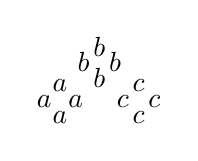
\begin{tikzpicture}
\draw (-0.5,0.0) node {$a$};
\draw (-0.7,0.2) node {$a$};
\draw (-0.3,0.2) node {$a$};
\draw (-0.5,0.4) node {$a$};
\draw (0.0,0.9) node {$b$};
\draw (0.2,0.7) node {$b$};
\draw (-0.2,0.7) node {$b$};
\draw (0.0,0.5) node {$b$};
\draw (0.5,0.0) node {$c$};
\draw (0.7,0.2) node {$c$};
\draw (0.3,0.2) node {$c$};
\draw (0.5,0.4) node {$c$};
\end{tikzpicture}

\end{center}

The rules of $\mathcal{F}$ enable us to make judgements about the objects of
$\mathcal{F}$. A judgement is a statement about some objects of $\mathcal{F}$,
which holds if it can be inferred from the rules of $\mathcal{F}$.  Judgements
come in various forms, judging over a number of objects. For instance, given
the objects $n$, $n_1$, and $n_2$, we may consider, among others, the following
forms of judgement:

\begin{table}[h]
\centering
\begin{tabular}{|l|l|}
\hline
\textbf{Judgement form} & \textbf{Reading} \\
\hline
$n\;\text{nat}$ & $n$ is a natural number. \\
\hline
$n=n_1+n_2$ & $n$ is the sum of $n_1$ and $n_2$.\\
\hline
\end{tabular}
\end{table}

% hypothetical judgement

The rules of $\mathcal{F}$ are rules of inference, dealing in judgements. A
rule is a relation between some judgements, called its premises, and a
judgement, called its conclusion\footnote{Although a set of premises may permit
us to infer multiple conclusions, we assume that they are inferred by different
rules.}. The rule, provided evidence that its premises hold, permits to infer
that the conclusion holds.

Let us adopt the common ``bar-notation'' for denoting rules, with the premises
of a rule presented above a horizontal line, and the conclusion below. For
instance, given the symbols $\symb{z}$ (read: zero) and $\symb{s}$ (read:
successor), we may consider the judgement $n\;\text{nat}$ to be defined as
follows:

\begin{equation}\label{natz-rules}
\sequent[NatZ-Zero]{}{\symb{z}\;\text{nat}}
\quad
\sequent[NatZ-Rec]{n\;\text{nat}}{{\symb{s}n\;\text{nat}}}
\end{equation}

Informally, these rules state that a natural number is either zero, or a
successor of a natural number.

Rules without premises are typically called axioms in that they hold
unconditionally. For instance, zero is always a natural number by the
\ruleref{Nat-Zero} axiom. The conclusion of one rule may form a premise of
another, perhaps the same, rule. This permits us to combine rule applications
into proofs of judgements. A proof is a witness that the judgement holds.

For instance, \ref{natz-rules} permits us to make the judgement
$\symb{s}\symb{s}\symb{s}\symb{z}\;\text{nat}$:

$$
\sequent{
  \sequent{
    \sequent{
      \sequent{
      }{\symb{z}\;\text{nat}}
    }{\symb{s}\symb{z}\;\text{nat}}
  }{\symb{s}\symb{s}\symb{z}\;\text{nat}}
}{\symb{s}\symb{s}\symb{s}\symb{z}\;\text{nat}}
$$

An object may be empty, that is, not consist of any symbols what-so-ever. For
instance, given some symbol $\bullet$ (read: star), we may consider the judgement
$n\;\text{nat}$ to be defined as follows:

\begin{equation}\label{nate-rules}
\sequent[NatE-Zero]{}{\;\text{nat}}
\quad
\sequent[NatE-Rec]{n\;\text{nat}}{\bullet n\;\text{nat}}
\end{equation}

Informally, these rules state that a natural number is either the empty object,
or a $\bullet$ followed by a natural number. Meaning that we can deduce which
natural number (in the classical sense) a natural number in $\mathcal{F}$
represents by counting the number of $\bullet$s. For instance, \ref{nate-rules}
permits us to make the judgement $\bullet\bullet\bullet\;\text{nat}$:

$$
\sequent{
  \sequent{
    \sequent{
      \sequent{
      }{\;\text{nat}}
    }{\bullet\;\text{nat}}
  }{\bullet\bullet\;\text{nat}}
}{\bullet\bullet\bullet\;\text{nat}}
$$

Empty objects can be a bit cryptic however, as they are not clearly
distinguished from other objects. It is convenient to adopt the following
notation:

\begin{definition}
Let $\varepsilon$ (read: epsilon) denote the empty object.
\end{definition}

\ref{nate-rules} can now be restated as follows:

\begin{equation}\label{nat-rules}
\sequent[Nat-Zero]{}{\varepsilon\;\text{nat}}
\quad
\sequent[Nat-Rec]{n\;\text{nat}}{\bullet n\;\text{nat}}
\end{equation}

Another informal reading of these rules is that a natural number is either the
empty sequence, or a sequence of $\bullet$s. Such a representation is
convenient as we can determine which natural number (in the classical sense)
$n\;\text{nat}$ represents by counting the number of $\bullet$s in $n$.

As another example, let the judgement $s\;\text{bitseq}$, reading $s$ is a
binary digit (bit) sequence, be defined as follows:

\begin{align}\label{bitseq-rules}
\begin{array}{c}
\sequent[BitSeq-Zero]{}{\varepsilon\;\text{bitseq}}
\\ \\
\sequent[BitSeq-Rec0]{s\;\text{bitseq}}{\symb{0} s\;\text{bitseq}}
\quad
\sequent[BitSeq-Rec1]{s\;\text{bitseq}}{\symb{1} s\;\text{bitseq}}
\end{array}
\end{align}

Informally, these rules state that a bit sequence is either the empty sequence,
or a sequence of bits (\symb{0} or \symb{1}).

The rules of \ref{nat-rules} and \ref{bitseq-rules} bear a lot of resemblance.
Both permit the sequencing of symbols chosen from an alphabet. Such sequencing
will be frequent throughout the thesis and so we define a generalized recursor
for it:

\begin{definition}

Given a judgement $w\;\Sigma$, let the judgement $s\;\Sigma^*$ be defined as
follows:

\begin{equation}\label{star-rules}
\sequent[Star-Zero]{}{\varepsilon\;\Sigma^*}
\quad
\sequent[Star-Rec]{
  w\;\Sigma \quad s\;\Sigma^*
}{
  w s\;\Sigma^*}
\end{equation}

\end{definition}

For instance, let $w\;\text{bullet}$ be defined as follows:

\begin{equation}
\sequent{}{\bullet\;\text{bullet}}
\end{equation}

\begin{theorem}
$s\;\text{bullet}^* \Leftrightarrow s\;\text{nat}$.
\end{theorem}

\begin{proof} Each direction by induction on the structure of $s$.. \end{proof}

Similarly, let $w\;\text{bit}$ be defined as follows:

\begin{equation}
\sequent{}{\symb{0}\;\text{bit}}
\quad
\sequent{}{\symb{1}\;\text{bit}}
\end{equation}

\begin{theorem}
$s\;\text{bit}^* \Leftrightarrow s\;\text{bitseq}$.
\end{theorem}

\begin{proof} Each direction by induction on the structure of $s$.. \end{proof}

Next: for each $s\;\Sigma^*$, there is a unique $n\;\text{nat}$ (recursive
enumerability).

\newpage

% The rules of a formal system may fall into a number of different classes. The
% class of \textbf{formation rules} consists of the rules governing how we can
% combine the symbols of the system to form \textbf{formulas}. The rest of the
% rules

% reasonably verifiable

% formal systems allow to state a problem
% the rules of a formal system allow to solve the problem

Formal systems are a purely mental construct. To be used to any effect in the
material world, a formal system must be realised by a physical system.

% Within our current understanding of the physical world, formal systems are an
% idealised construct. A \textbf{physical system} is subject to the laws of
% physics and other real-world constraints. Formal systems enjoy the freedom of
% the immaterial world.

% formal systems are specifications such that not only are they reasonably
% realisable, but also the adherence of the realisation to the specification is
% reasonably verifiable.

\begin{notion}

A physical system, $\mathcal{P}$, is a system of physical symbols and processes
manipulating them.

\end{notion}

$\mathcal{P}$ can be a reasonable realisation of formal system $\mathcal{F}$,
provided that\begin{inparaenum}[(1)]\item there is a reasonable correspondence
between the symbols of $\mathcal{F}$ and the physical symbols of $\mathcal{P}$,
and \item $\mathcal{P}$ manipulates the physical symbols in reasonable
accordance with the rules of $\mathcal{F}$\end{inparaenum}. For instance, this
report is (hopefully) a reasonable realisation of the formal systems that the
author had in mind.

If $\mathcal{P}$ is a reasonable realisation of $\mathcal{F}$, $\mathcal{F}$
can serve to specify the desired (or perceived) behaviour of $\mathcal{P}$.
Such a specification becomes useful in communicating how a physical system is
to be employed to solve a real-world problem.

\begin{notion}

$\mathcal{F}$ \textbf{solves} a problem $P$, if $P$ can be stated as formula
$f$ in $\mathcal{F}$, and after a finite sequence of symbolic manipulations
legal for $\mathcal{F}$, we arrive at a formula $f'$, which can be deemed a
statement of a solution to $P$.

\end{notion}

\pagebreak

Formal systems, and so their realisations, bear little intrinsic purpose ---
symbolic manipulation is a means to an end for more purposeful beings. In how
far a realisation is reasonable, is therefore a matter of the intended
\textbf{purpose} of the system.

\begin{notion}

A formal system $\mathcal{F}$ can solve a \textbf{problem} $P$, if $P$ can be
expressed with the symbols of $\mathcal{F}$, in accordance to the rules of
$\mathcal{F}$, 

\end{notion}

A system specification is useful to more purposeful beings for communicating
how a system can be used to solve a particular problem. The class of problems
which can be solved by rote symbolic manipulation is the class of
\textbf{computable} problems.

\begin{definition}

A problem is \textbf{computable} if it can be solved by performing a sequence
of symbolic manipulations.

\end{definition}

\begin{definition}

A \textbf{derivation} is a sequence of rule applications.

\end{definition}

\newpage

Formal
systems in this regard, become useful in communicating how a physical system is
to be used to solve a particular problem.


Physical systems realising formal systems are often referred to as
\textbf{computers}, and the activity of symbolic manipulation as
\textbf{computation}.

Before the mid-20th century, computation was generally the faculty of human
beings, with the help of paper and pencil, and perhaps, an abacus. With the
whirlwind of world history, human realisation of formal systems became
unreasonable, and we turned to computation by machines, less prone to err,
defect, or betray, and much faster at it.

This has allowed us to deal in a range of formal systems which we can
reasonably assume to be \textbf{absolutely realisable}, i.e. having physical
realisations which do not deviate from their formal specification. For
instance, we can reasonably assume that the Intel(R) Core(TM) i7-4600U
processor performs computation in accordance with its data sheet.

Dealing in absolutely realisable formal systems directly has proven a challenge
however.

As formal systems are a means to an end for more purposeful beings, we are not
only concerned with employing a formal system, 

This turn allowed for an elevation from much concern about physical
realisation, and today we generally assume that modern computers absolutely
realise the formal systems that specify them. As a result, the field of
Computer Science is generally concerned with\begin{inparaenum}[(1)]\item what
can be solved using formal systems, with \textbf{reasonable elegance} \item,
while \item staying within the realm of reasonable
realisability\end{inparaenum}.

To comply with (3), ... 

Much like a physical system can realise a formal system, a formal system
$\mathcal{G}$ can realise a formal system $\mathcal{F}$. This is usually
referred to as a \textbf{simulation}.

\begin{definition}

A formal system $\mathcal{F}=\chev{\mathcal{F}_S,\mathcal{F}_R}$ can be
simulated by a formal system $\mathcal{G}=\chev{\mathcal{G}_S,\mathcal{G}_R}$,
provided that\begin{inparaenum}[(1)]\item there is a 1-1 correspondence between
the $\mathcal{F}_S$ and $\mathcal{G}_S'$, where
$\mathcal{G}_S'\subseteq\mathcal{G}_S$, and \item $\mathcal{G}_R$ allow to
manipulate $\mathcal{G}_S'$ in accordance with $\mathcal{F}_R$\end{inparaenum}.

\end{definition}

% Desired for the formal system: consistent & complete
% Desired for the physical system: reliable, i.e. accurate.





\section{Audience} \label{sec:introduction:audience}

The audience of this thesis is anyone interested in the connection of
computability and complexity to the theory and practice of programming
languages.

In particular, what the admittance of useful programming language constructs
implies for the time and space complexity of the programs that you can write. A
programming language construct is ``useful'' if its admission permits to write
a practical class of programs in an elegant manner.

The thesis is directed towards the level of a Computer Science graduate student
at the time of writing: The reader is assumed to be familiar with the basics of
discrete mathematics, as in \cite[\ch~0]{sipser-2013}, and \cite[Appendices A,
B, and C]{cormen-et-al-2009}. The analysis of time and space complexity of
algorithms, as in \cite[\chs~1--17 and \chs~21--24]{cormen-et-al-2009}. Regular
and context-free languages, as in \cite[\chs~1--2]{sipser-2013}, and their use
for programming language design, as in \cite{mogensen-2010}. The reader should
also be familiar with Logic in Computer Science, as in
\cite[\chs~1--4]{huth-ryan-2004}.


% vim: set spell:

\section{Preliminaries}

\begin{definition} Let $\mathbb{N}$ denote the type of natural numbers,
including $0$. \end{definition}

\begin{definition} Given a type $\Sigma$, let $\Sigma^*$ be the type of
\textbf{symbolic strings} over $\Sigma$, formed using either the \textbf{empty
string} or the \textbf{string concatenation} operator:
\begin{align*}\label{def:empty-string}
\judgement{}{\varepsilon_\Sigma:\Sigma^*}
\quad
\judgement{s_0:\Sigma \quad s:\Sigma^*}{s_0 \cdot s:\Sigma^*}
\end{align*}
We refer to $\Sigma$ as an \textbf{alphabet}, and to the terms of $\Sigma$ as
\textbf{symbols}. \end{definition}

We omit $\Sigma$ in $\varepsilon_\Sigma$, when it is clear from context, e.g.
$\varepsilon:\Sigma^*$.

\begin{definition} We say that a term $s\equiv s_0 \cdot s_1 \cdots s_{n-1}
\cdot \varepsilon : \Sigma^*$  is a string of length $n:\mathbb{N}$ over the
alphabet $\Sigma$.\end{definition}

\begin{definition} Let $\card{\Sigma}$ be the number of symbols in alphabet
$\Sigma$, called it's \textbf{cardinality}. \end{definition}

If the cardinality of an alphabet is finite, strings over the alphabet are
\textbf{recursively enumerable}, i.e. there exists a bijection
$f:\Sigma^*\rightarrow\mathbb{N}$.

\begin{theorem} If $\card{\Sigma} = n$ for some $n\in\mathbb{N}$, then
$\card{\Sigma^*}=\card{\mathbb{N}}$.\end{theorem}

\begin{proof} We have $\card{\Sigma} = n$. The terms of $\Sigma$ can be
arranged in a sequence such that for each $s:\Sigma$ we assign a unique natural
number $g(s)$, such that $1 \leq g(s) \leq \card{\Sigma}$. We now inductively
define the function $f:\Sigma^*\rightarrow \mathbb{N}$.

\begin{align}
f\p{\varepsilon} &= 0 \\
f\p{s_0\cdot s} &= g\p{s_0} + f\p{s} \cdot \card{\Sigma}
\end{align}

To show that the function is a bijection, we also define its inverse by
induction:

\begin{align}
f^{-1}\p{0} &= \varepsilon \\
f^{-1}\p{n} &= g^{-1}\p{n \mod \card{\Sigma}} \cdot f^{-1}\p{\floor{n/\card{\Sigma}}} & \text{for $n>0$}
\end{align}

\end{proof}

This means that strings over any finite alphabet can be used to represent
strings over any other finite alphabet. One such basic alphabet that has proven
useful in practice is the binary alphabet, consisting of e.g. the symbols
\texttt{0} and \texttt{1}.

\begin{definition} Let $\mathbb{B}$ denote the type of booleans.\end{definition}

Define the set $\mathbb{B}$, and the usual boolean connectives.

\begin{definition} An infix function $\leq : A\times A \rightarrow \mathbb{B}$ defines a
\textbf{total order} on the type $A$ iff for all $x,y,z : A$:
\begin{align}
x \leq y \wedge y \leq x \Rightarrow y = x  & \quad \text{(antisymmetry)} \\
x \leq y \wedge y \leq z \Rightarrow x \leq z & \quad \text{(transitivity)} \\
x \leq y \vee y \leq x & \quad \text{(totality)}
\end{align}
\end{definition}

\begin{definition} Given a total order on $\Sigma$, we define the
\textbf{lexicographic order} on $\Sigma^*$ as follows:
\begin{align}
\judgement{}{\varepsilon \leq s_0\cdot s}
\quad
\judgement{s_0 = t_0 \quad s \leq t}{s_0\cdot s \leq t_0 \cdot t}
\quad
\judgement{s_0 \neq t_0 \quad s_0 \leq t_0}{s_0 \cdot s \leq t_0 \cdot t}
\end{align}
\end{definition}

\begin{theorem} A lexicographic order is a total order. \end{theorem}

\begin{proof} \end{proof}

\begin{definition} An infix function $<:A\times A \rightarrow \mathbb{B}$
defines a \textbf{strict total order} on the type $A$, iff 
\begin{align}
\judgement[F-Less]{\neg \p{y \leq x}}{x < y}
\end{align}
\end{definition} 

We say that $y$ has a higher \textbf{value} than $x$, whenever $x<y$, and equal
in value whenever $x=y$.

\begin{definition} A function $f$ is defined by \textbf{primitive recursion}
from the functions $g,h_1,h_2,\ldots,h_n$ for $n:\mathbb{N}$, iff
\begin{align}
f\p{\varepsilon, \vect{y}} &= g\p{\vect{y}} \\
f\p{s_i\p{x}, \vect{y}} &= h_i\p{x,\vect{y},f\p{x,\vect{y}}} \\
x &< s_i\p{x}
\end{align}
\end{definition}

That is, a function is defined by primitive recursion, if on every invocation
of the function, we recurse on at most one formal parameter, and only recurse
after the actual parameter has been decreased in value. It follows that
primitive recursion demands a strict total order on the value type in question.

\begin{definition} A function is \textbf{primitive recursive} if it is
non-recursive, or defined by primitive recursion from non-recursive, or
primitive recursive functions.  \end{definition}

Primitive recursive functions are not necessarily polytime functions.

\begin{example}
Unary addition over binary notation is primitive recursive, but not polytime.

Let $\leq$ be the lexicographic order on binary notation.

We now define unary addition over binary notation using primitive recursion:

\begin{align}
add'\p{0,0,0} = \p{0,0} \\
add'\p{1,0,0} = \p{1,0} \\
add'\p{0,1,0} = \p{1,0} \\
add'\p{0,0,1} = \p{1,0} \\
add'\p{0,0,1} = \p{1,0} \\
add'\p{1,1,0} = \p{0,1} \\
add'\p{1,1,1} = \p{1,1}
\end{align}

\end{example}

